\section{Simulations of Detector Performance}

Extensive Monte Carlo simulations were carried out as part of the detector
design procedures. This section describes some of the features of the 
expected detector performance based on the current design.

\subsection{Optical Properties of Physical Components}

The criterion for the choice of physical components is to maximize the
production and detection of electron {\v C}erenkov light with the maximum 
threshold energy for pion {\v C}erenkov radiation.  Fig.~\ref{transparancy} 
is a composite showing the properties of the various materials that
play important roles in the {\v C}erenkov performance. 

%%%%%%%%%%%%%%%%%%%%%%%%%%%%%%%%%%%%%%%%%%%%%%%%%%%%%%%%%%%%%%%%%%%%%%
\begin{figure}[htbp]
\centering
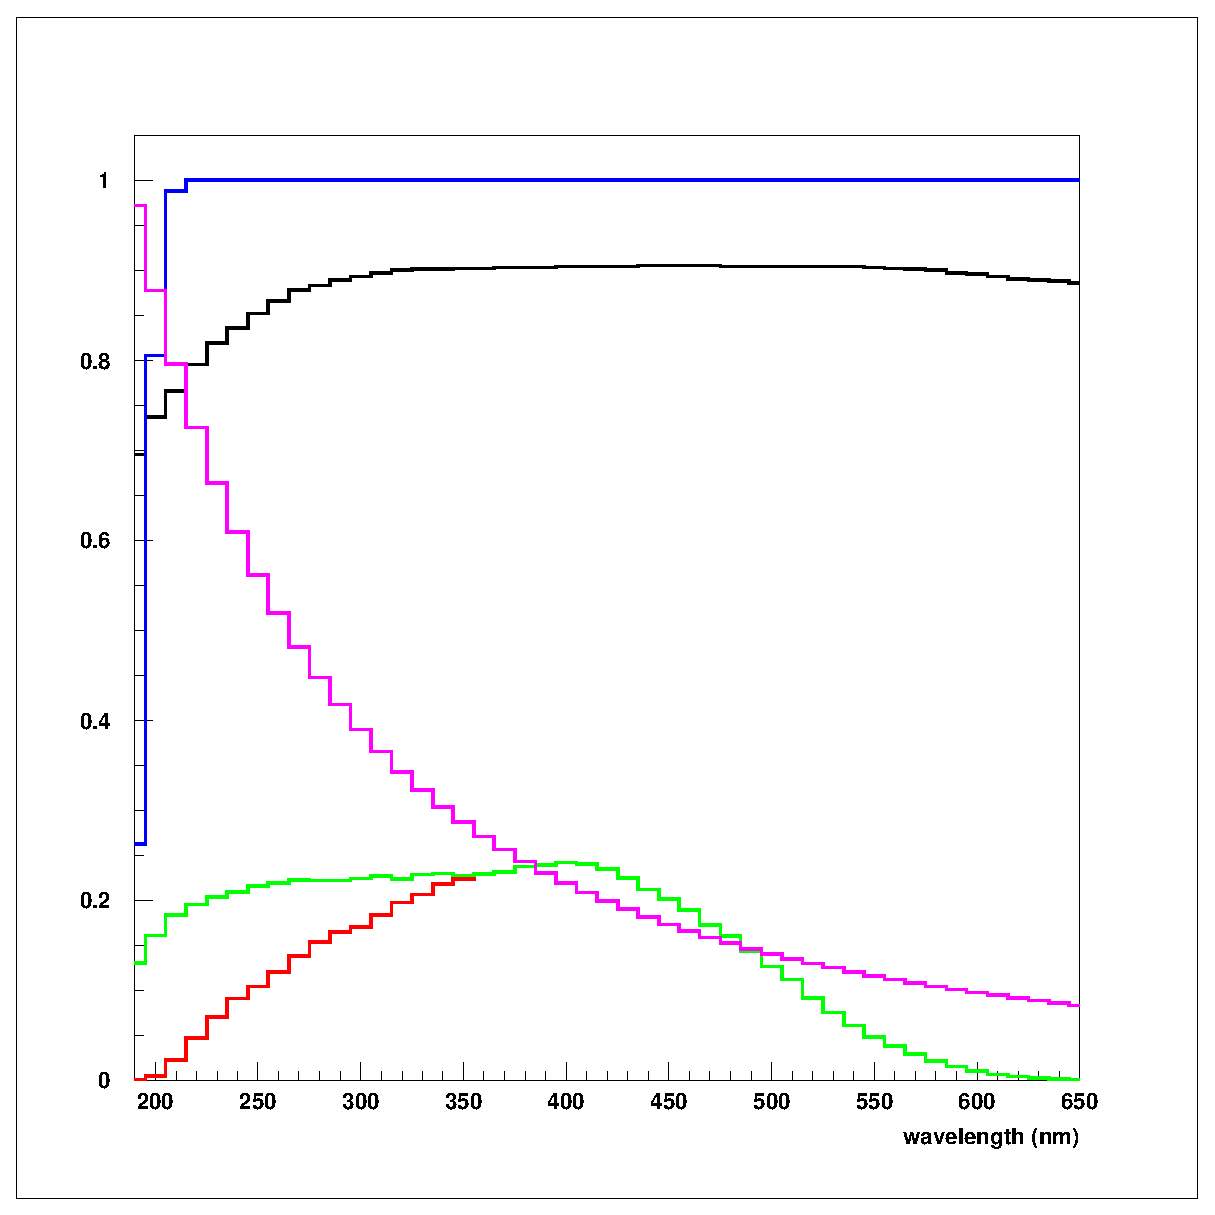
\includegraphics[height=12cm,angle=0]{MC-simulation/nphe_calc.eps}
\caption{\small{The optical properties of components of the HTCC
relative to maximizing the number of detected photoelectrons
as a function of photon wavelength.  The transparency of CO$_2$ is 
shown in blue, the reflectivity of aluminum in black, the photo-efficiency 
of a PMT with a UV glass window in red, and a quartz window in green. 
The magenta line represents the {\v C}erenkov spectrum (in arbitrary 
units).}}
\label{transparancy}
\end{figure}
%%%%%%%%%%%%%%%%%%%%%%%%%%%%%%%%%%%%%%%%%%%%%%%%%%%%%%%%%%%%%%%%%%%%%%

\subsubsection{Radiator Gas} 

The choice of radiator gas is CO$_2$, which has excellent optical 
transparency for wavelengths as low as 200~nm (see Fig.~\ref{transparancy}).
This is an important feature since the spectrum of {\v C}erenkov light is 
approximately $dn/d\lambda\propto 1/\lambda^2$.  The low index of 
refraction, $n \sim 1.00041$, corresponds to a pion threshold energy of 
4.7~GeV.  The trade-off is that fewer photons are produced at such low 
values of $n$. However, as will be seen, the number of collected photons 
is high enough to ensure a high detection efficiency. 

\subsubsection{Photomultiplier Tubes}

The use of 5-in photomultiplier tubes was chosen as the best match for the 
optical properties of the HTCC. This will be clear in the section on the 
photon spacial distributions at the face of the PMTs.  After consideration 
of PMTs from several manufacturers~\footnote{ElectronTubes, Burle, Hamamatsu, 
Photonis}, the Photonis XP4508 was chosen to have the best overall 
characteristics for our requirements. The window material is an important 
consideration.  Fig.~\ref{transparancy} compares the quantum efficiency of 
the Photonis XP4508 with UV glass and quartz windows. Clearly, the quartz 
window is superior in the low wavelength regime in which there are a large 
number of photons, and it matches the transparency range of the CO$_2$, as 
well as the reflectivity of the Al-MgF$_2$ mirror surfaces, which are also 
shown in Fig.~\ref{transparancy}.

The intensity and spectrum of \v{C}erenkov photons is given by the 
Frank-Tamm relation:

\begin{equation}
\frac{dN_{\gamma}}{dE} = \left( \frac{\alpha}{\hbar c} \right) Z^2 L
\left[1-(\frac{1}{n(E)\beta})^2 \right],
\end{equation} 

\noindent
where $Z$ is the particle charge, $n(E)$ is the index of refraction,
$L$ is particle trajectory length, and $(\frac{\alpha}{\hbar c}) = 
370$~eV$^{-1}$cm$^{-1}$. The expected number of obtained photoelectrons 
is then:
   
\begin{equation}
N_{ph.e.} = \int {}{}  \frac{dN_\gamma} {dE} \varepsilon(E)dE,
\end{equation}

\noindent
where $\varepsilon(E)$ is the detection efficiency of photons with energy 
$E$.  $\varepsilon(E)$ depends on the {\v C}erenkov gas transparency, 
reflection losses, quantum sensitivity of the PMT, and the probability of
missing the PMT because of geometry factors.  

The calculated mean number of photoelectrons per 1~cm of the trajectory is 
0.1477 for a UV glass PMT window and 0.2086 for a quartz PMT window.  The 
difference is essentially because of the fact that the {\v C}erenkov photon 
spectrum has an enhancement at low wavelengths -- see 
Fig.~\ref{transparancy}.  For our Monte Carlo simulations we assume quartz 
PMT windows.  The number of obtained photoelectrons was corrected for 
mirror imperfections and possible misalignments.  The correction 
coefficient, derived from the ratio of the Monte Carlo simulations and 
the experimental number of photoelectrons for the CLAS LTCC, was equal to 
2/3.

The shape of the PMT surface has also been considered, since the 
reflectivity of the PMT window, and thus the quantum efficiency, depends 
on the distribution of the angles of the photons relative to the PMT 
surface.   Fig.~\ref{angles} shows the simulated distribution of photon 
angles relative to the normal to the PMT surface for convex and flat 
windows, respectively.  It is seen that the distribution for the flat 
surface is closer to the surface normal than for the convex surface, and 
thus the flat surface quartz window was chosen as most appropriate for our 
purposes.

%%%%%%%%%%%%%%%%%%%%%%%%%%%%%%%%%%%%%%%%%%%%%%%%%%%%%%%%%%%%%%%%%%%%%%
\begin{figure}[htbp]
\centering
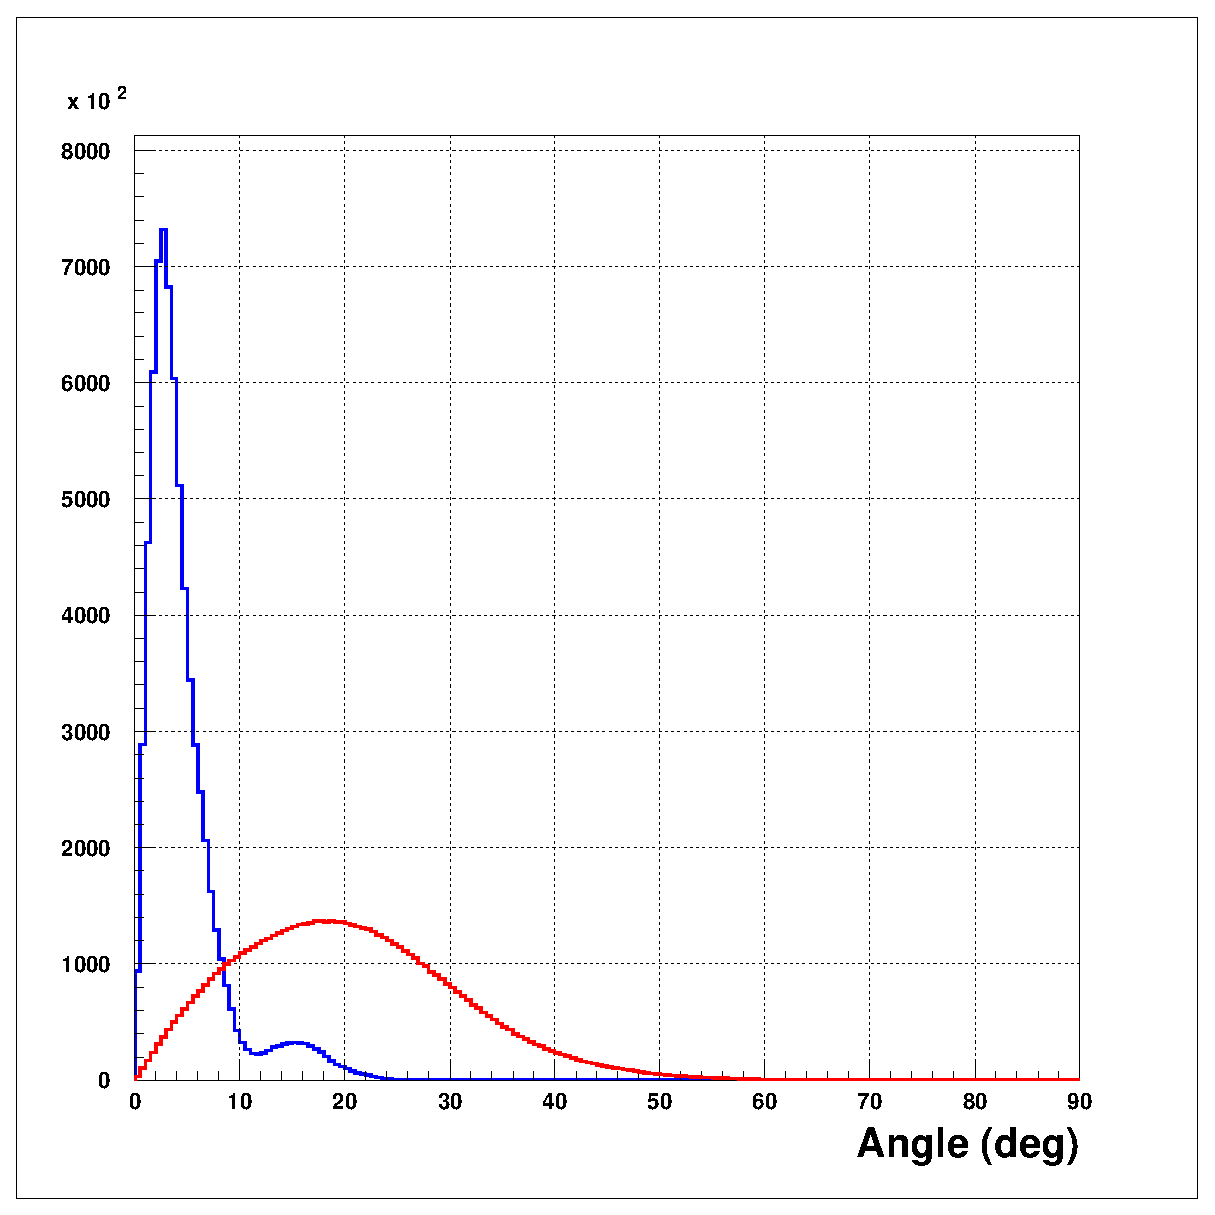
\includegraphics[height=8cm,angle=0]{MC-simulation/angles.eps}
\caption{\small{The simulated distribution of photon angles relative to 
the normal to the PMT surface for convex (red) and flat (blue) windows, 
respectively. The enhancement near the 15$^\circ$ (blue curve) is due to 
the photons, reflected off the Winston cone.}}
\label{angles}
\end{figure}
%%%%%%%%%%%%%%%%%%%%%%%%%%%%%%%%%%%%%%%%%%%%%%%%%%%%%%%%%%%%%%%%%%%%%%

\subsection{Distributions of Photons Incident on the PMT Faces}

Simulations were carried out to assess the HTCC response to scattered
electrons as a function of scattering angle in both $\theta$ and $\phi$.  
The results discussed in this section are for electrons of energy 2~GeV 
uniformly distributed in $d\Omega=\cos \theta d\theta d\phi$.  Each mirror 
is designed to direct the {\v C}erenkov light that impinges upon it onto 
the face of a specific PMT.  Fig.~\ref{four-tubes} shows the distribution 
of photons reaching PMTs in the PMT surface plane. 

The electrons originate from a target of length 10~cm, which is centered at 
the nominal central target position, with the full magnetic field 
configuration.  It is observed that the photons are constrained to circles 
of diameter approximately 16~cm, which is somewhat larger than the 11~cm 
PMT active diameters. Thus, light collection cones (Winston Cones) have 
been designed to redirect the photons that arrive outside of the 
photosensitive areas of the PMTs into the photosensitive areas.  All 
calculations were made for a Winston Cone window diameter of 7.5~in. 

%%%%%%%%%%%%%%%%%%%%%%%%%%%%%%%%%%%%%%%%%%%%%%%%%%%%%%%%%%%%%%%%%%%%%%
\begin{figure}[htbp]
\centering
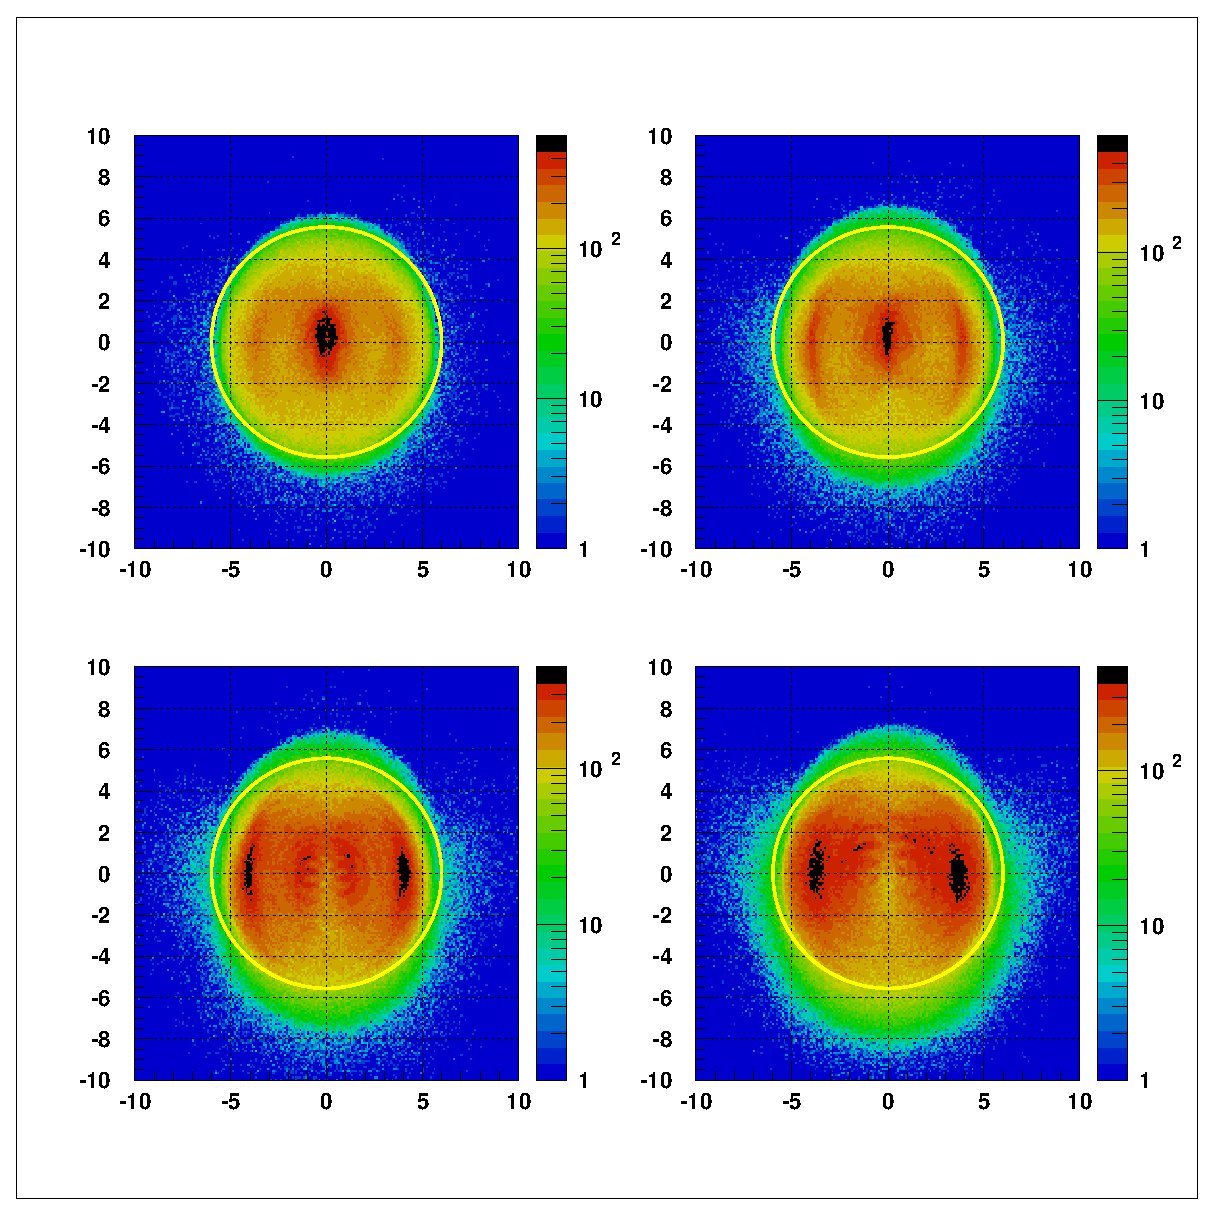
\includegraphics[height=14cm,angle=0]{MC-simulation/all_pmt.eps}
\caption{\small{The distribution of photons reaching the PMTs in the PMT
surface plane. Circles show the PMT size.}}
\label{four-tubes}
\end{figure}
%%%%%%%%%%%%%%%%%%%%%%%%%%%%%%%%%%%%%%%%%%%%%%%%%%%%%%%%%%%%%%%%%%%%%%

Fig.~\ref{nph-accept-2d} shows the overall acceptance in the number of 
photoelectrons as a function of $\theta$ and $\phi$ for one half of a 
sector, corresponding to the {\it standard} conditions described above. 
The results are the same for the 12 symmetrically placed half sectors 
corresponding to full $\Delta\phi = 2 \pi$.  Fig.~\ref{nph-vs-theta-phi} 
shows the projections of Fig.~\ref{nph-accept-2d} vs. $\theta$ and $\phi$,
respectively.  One observes that the mean number of photoelectrons is 
greater than 10 for scattered electrons in the angular range from about 
$5^\circ$ to $36^\circ$.  The $\theta$ dependence of the photoelectron 
number reflects the trajectory length dependence.

%%%%%%%%%%%%%%%%%%%%%%%%%%%%%%%%%%%%%%%%%%%%%%%%%%%%%%%%%%%%%%%%%%%%%%
\begin{figure}[htbp]
\centering
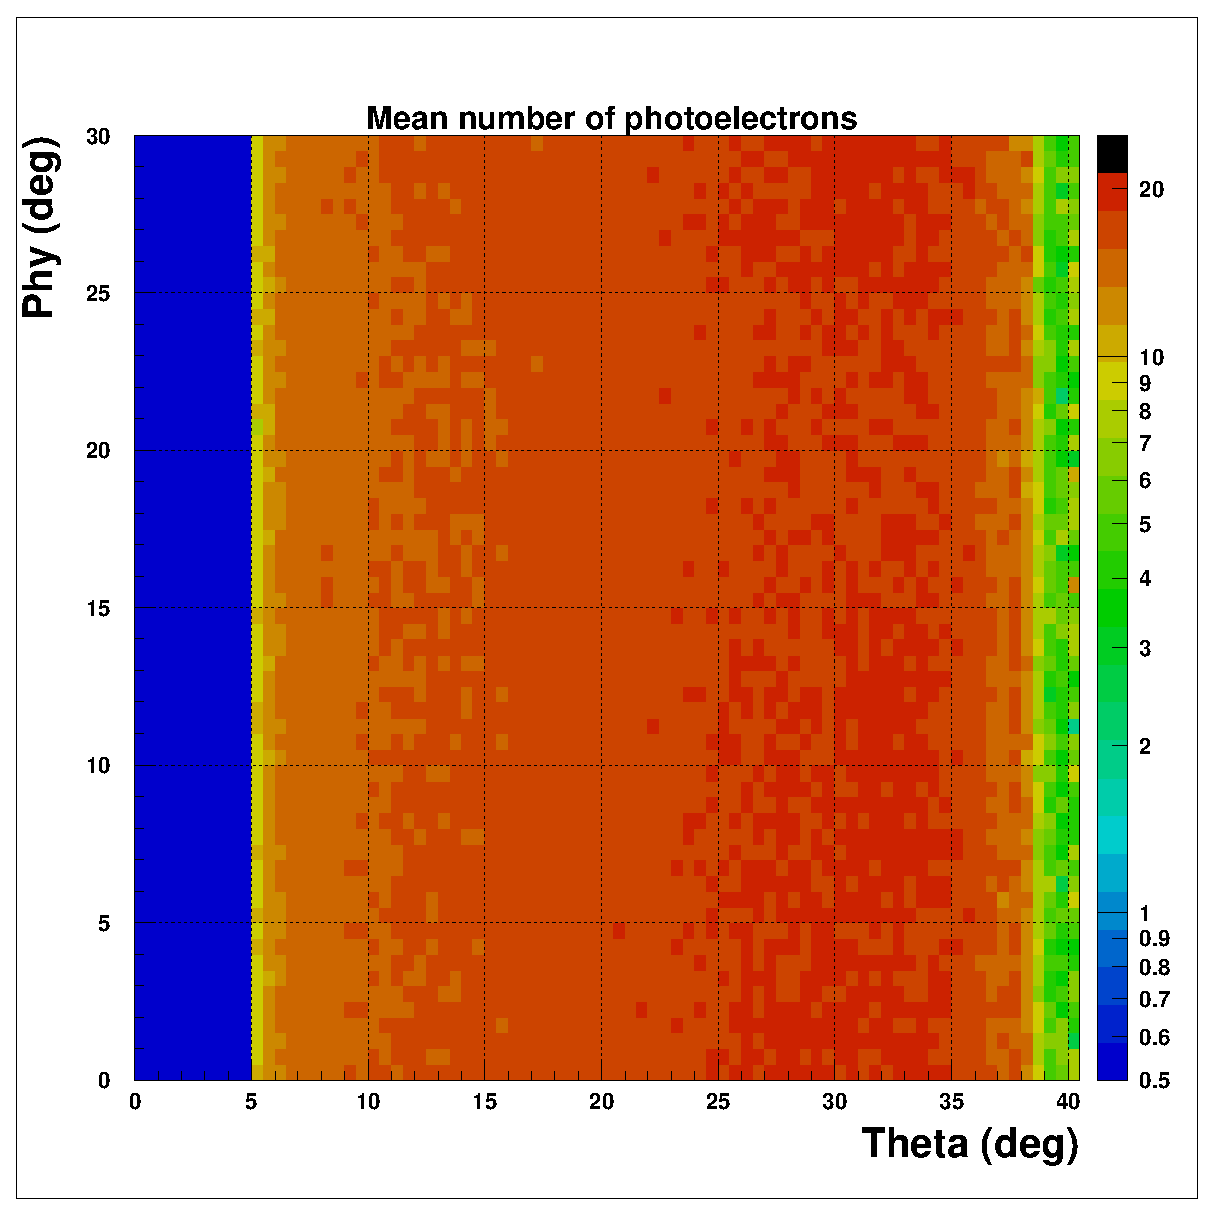
\includegraphics[height=12cm,angle=0]{MC-simulation/nph-accept-2d.eps}
\caption{\small{The overall acceptance in the number of photoelectrons
as a function of $\theta$ and $\phi$ for one half of a sector.}}
\label{nph-accept-2d}
\end{figure}
%%%%%%%%%%%%%%%%%%%%%%%%%%%%%%%%%%%%%%%%%%%%%%%%%%%%%%%%%%%%%%%%%%%%%%

%%%%%%%%%%%%%%%%%%%%%%%%%%%%%%%%%%%%%%%%%%%%%%%%%%%%%%%%%%%%%%%%%%%%%%
\begin{figure}[htbp]
\centering
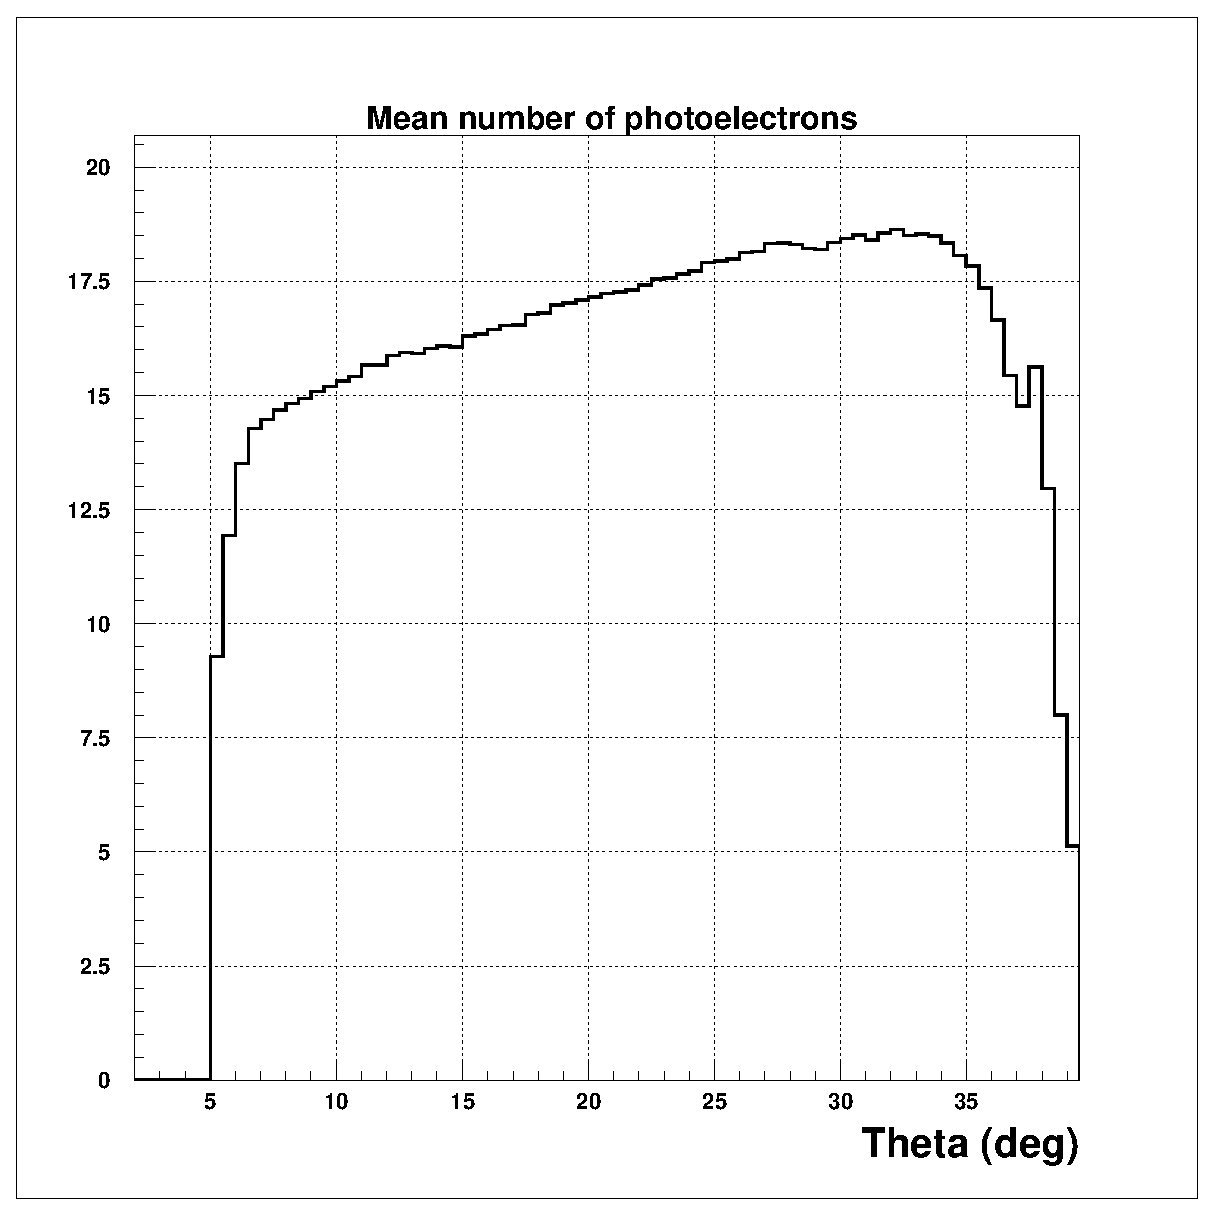
\includegraphics[height=8cm,angle=0]{MC-simulation/nph-vs-theta.eps}
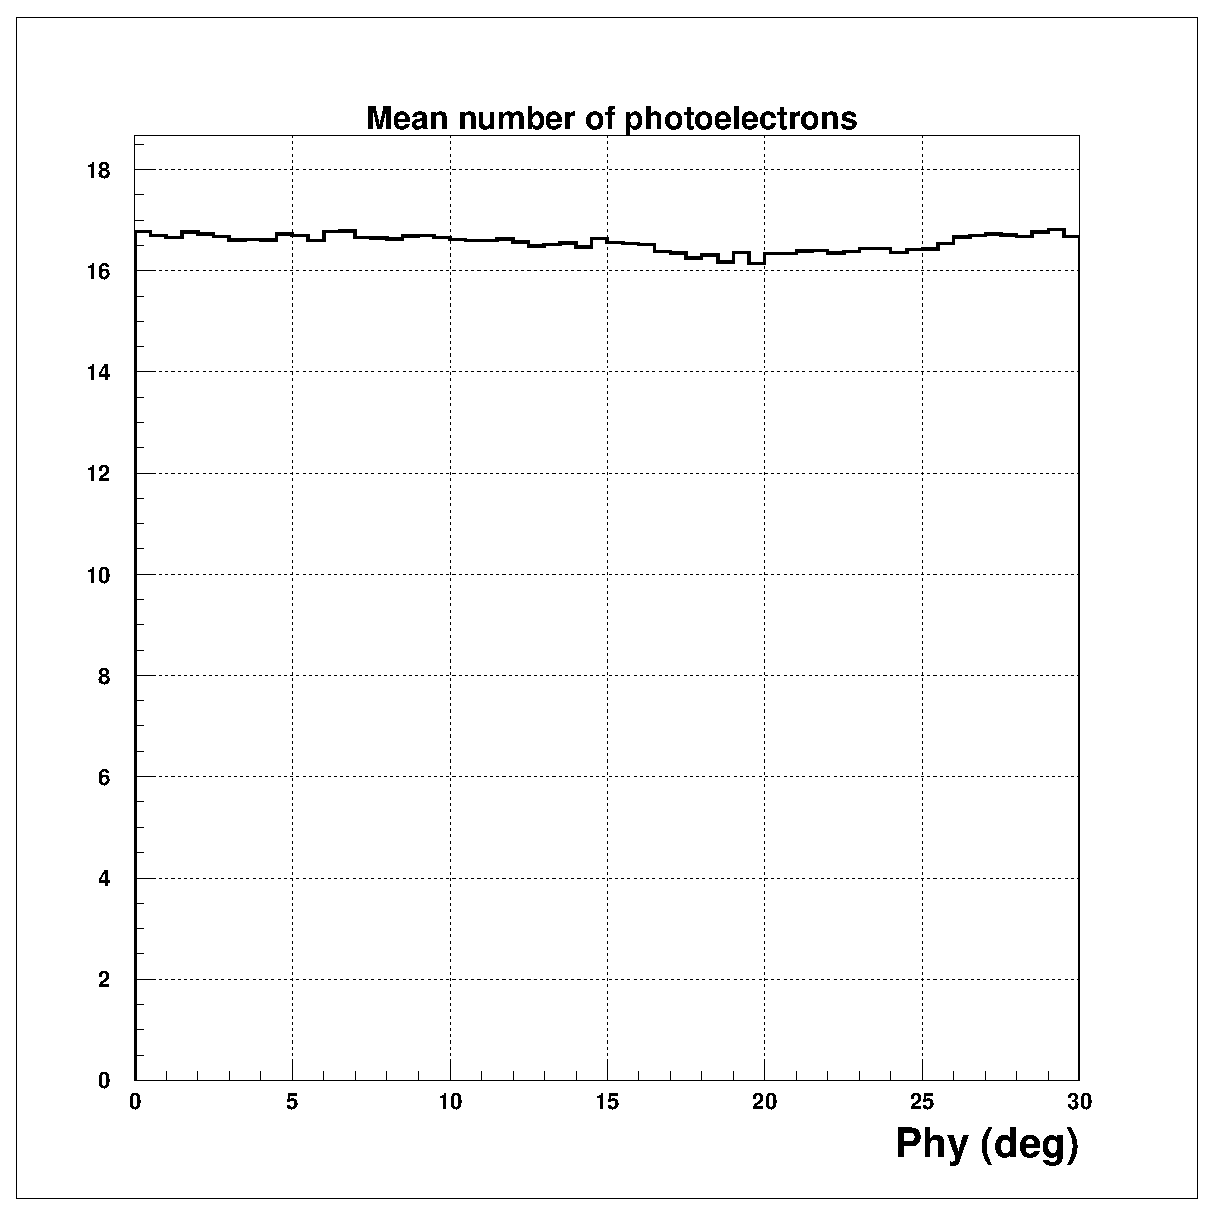
\includegraphics[height=8cm,angle=0]{MC-simulation/nph-vs-phi.eps}
\caption{\small{The projections of Fig.~\ref{nph-accept-2d} vs. 
$\theta$ and $\phi$, respectively.}}
\label{nph-vs-theta-phi}
\end{figure}
%%%%%%%%%%%%%%%%%%%%%%%%%%%%%%%%%%%%%%%%%%%%%%%%%%%%%%%%%%%%%%%%%%%%%%

%%%%%%%%%%%%%%%%%%%%%%%%%%%%%%%%%%%%%%%%%%%%%%%%%%%%%%%%%%%%%%%%%%%%%%
\begin{figure}[htbp]
\centering
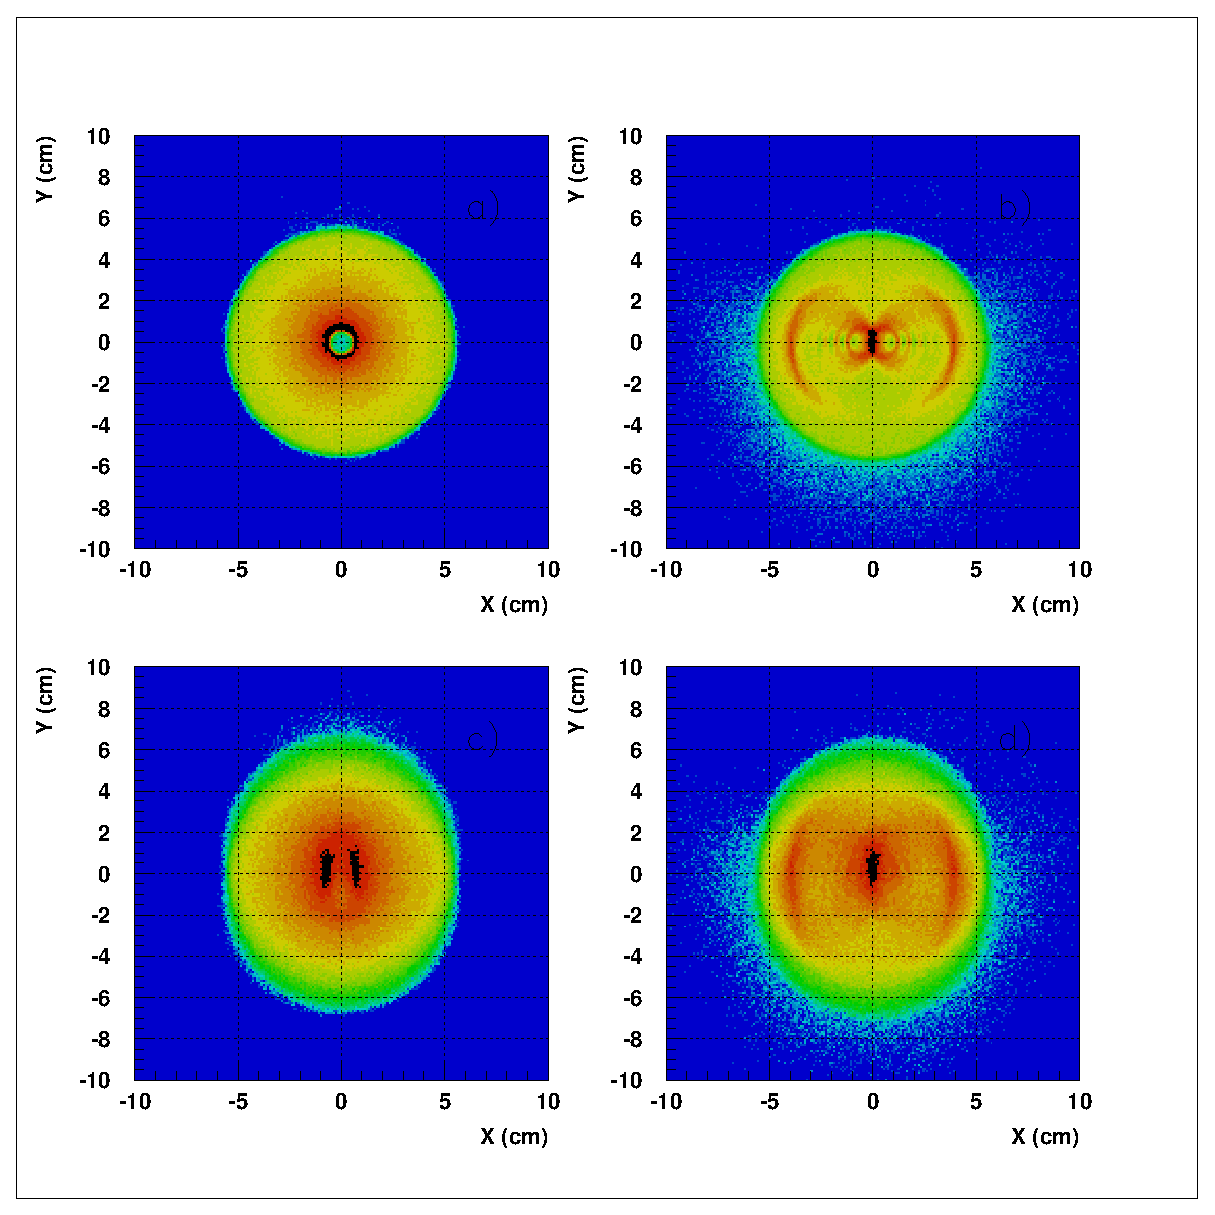
\includegraphics[height=12cm,angle=0]{MC-simulation/targ_field1.eps}
\caption{\small{The effect of the magnetic field and target length on the 
performance of the detector.  (a) is a point-like target, no magnetic field; 
(b) 10-cm target, no magnetic field; (c) and (d) are for a point-like target 
and a 10-cm target, respectively, in the 5~T solenoid magnetic field.}}
\label{fields}
\end{figure}
%%%%%%%%%%%%%%%%%%%%%%%%%%%%%%%%%%%%%%%%%%%%%%%%%%%%%%%%%%%%%%%%%%%%%%

The effect of the fields and target length on the performance of the 
detector are illustrated in Fig.~\ref{fields}a, b, c, and d, which show 
the distribution of photons on one PMT, number 2.  Case a) is a point-like 
target without magnetic field and case b) is a 10-cm target without magnetic 
field. Cases c) and d) are the point-like target and 10-cm target,
respectively, in the 5-T solenoid magnetic field.  Fig.~\ref{fields} shows 
that the distortions due to the target length and magnetic field are not 
very large, and the 7.5-inch diameter Winston Cone is an adequate choice
to collect all {\v C}erenkov light.

\subsection{Background Rates}

GEANT was used to estimate the background rate due to scattered electrons,
and electrons and positrons from secondary interactions with the detector 
materials.  Initial electrons with energy 11~GeV interact with the 5-cm 
liquid-hydrogen target in the 5-T solenoid magnetic field.  The beam pipe 
shielding starts from about 40~cm from the target.  The beam pipe shielding 
is between $2^\circ$ and $4^\circ$.  The PMT rates were reduced to the 
standard luminosity at 11~GeV, $10^{35}$~cm$^{-2}$s$^{-1}$.  The beam pipe 
shielding material was tungsten.

%%%%%%%%%%%%%%%%%%%%%%%%%%%%%%%%%%%%%%%%%%%%%%%%%%%%%%%%%%%%%%%%%%%%%%
\begin{figure}[htbp]
\centering
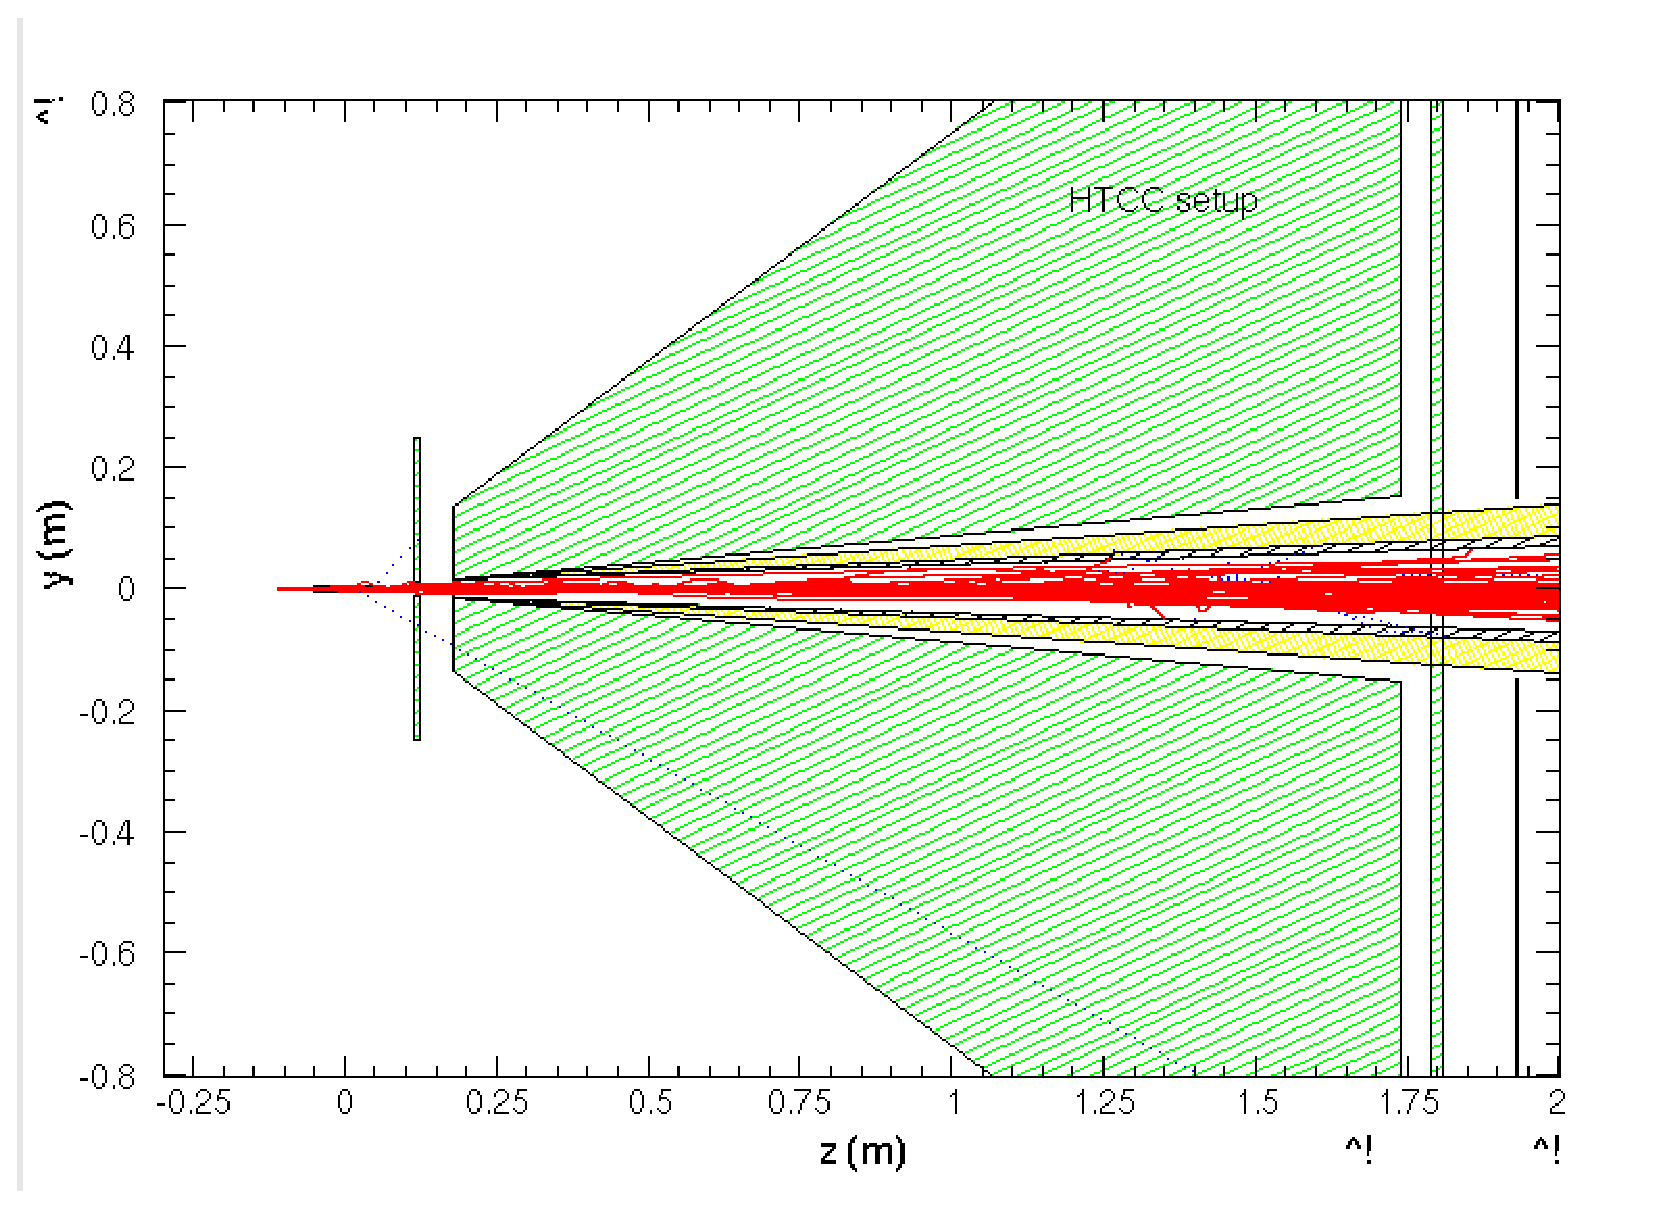
\includegraphics[height=6cm,angle=0]{MC-simulation/setup12.eps}
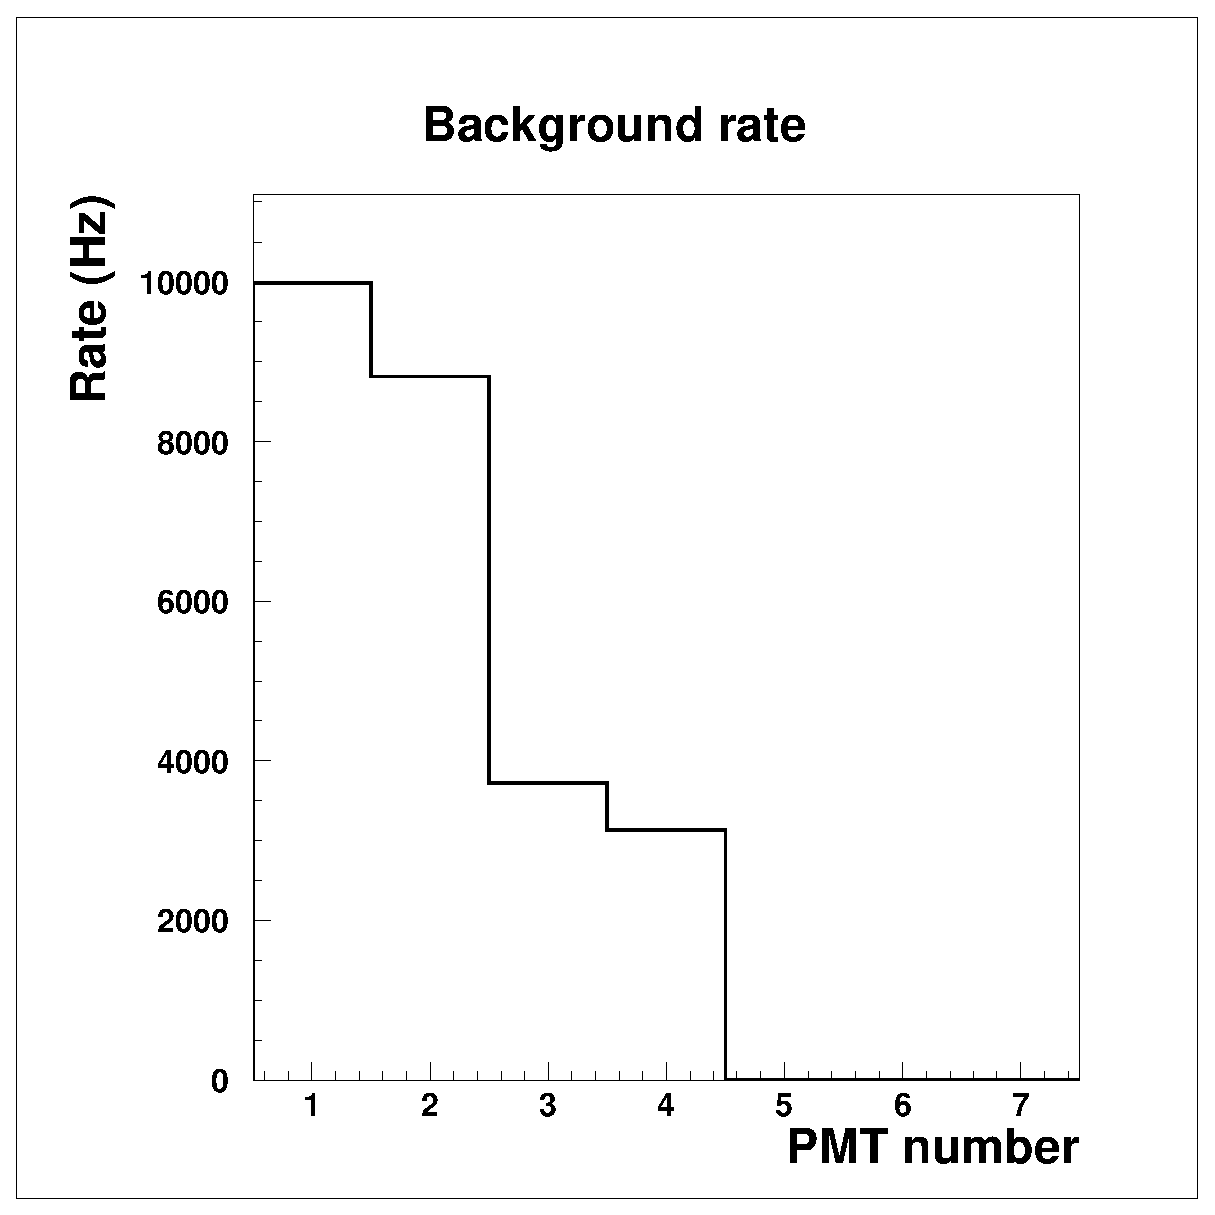
\includegraphics[height=6cm,angle=0]{MC-simulation/backgr1.eps}
\caption{\small{The experimental setup and background rates estimate.}}
\label{background1}
\end{figure}
%%%%%%%%%%%%%%%%%%%%%%%%%%%%%%%%%%%%%%%%%%%%%%%%%%%%%%%%%%%%%%%%%%%%%%

Fig.~\ref{background1} illustrates the beam pipe shielding setup and 
background PMT rates.  The highest rate is for the PMT at the lowest polar
angle.

For possible using the Inner Calorimeter for DVCS studies the other shielding
was designed. It covers the open angle from  $1^\circ$ to $1.5^\circ$,
and also the angle from  $5^\circ$ to $5.5^\circ$ . The setup and the
estimated background rate in this case is shown  in Fig.~\ref{background2}.
The background rate is a bit higher in this case, but
it can be easily handled by the data acquisition system.

 
%%%%%%%%%%%%%%%%%%%%%%%%%%%%%%%%%%%%%%%%%%%%%%%%%%%%%%%%%%%%%%%%%%%%%%
\begin{figure}[htbp]
\centering
\includegraphics[height=6cm,angle=0]{MC-simulation/dvcs12setup.eps}
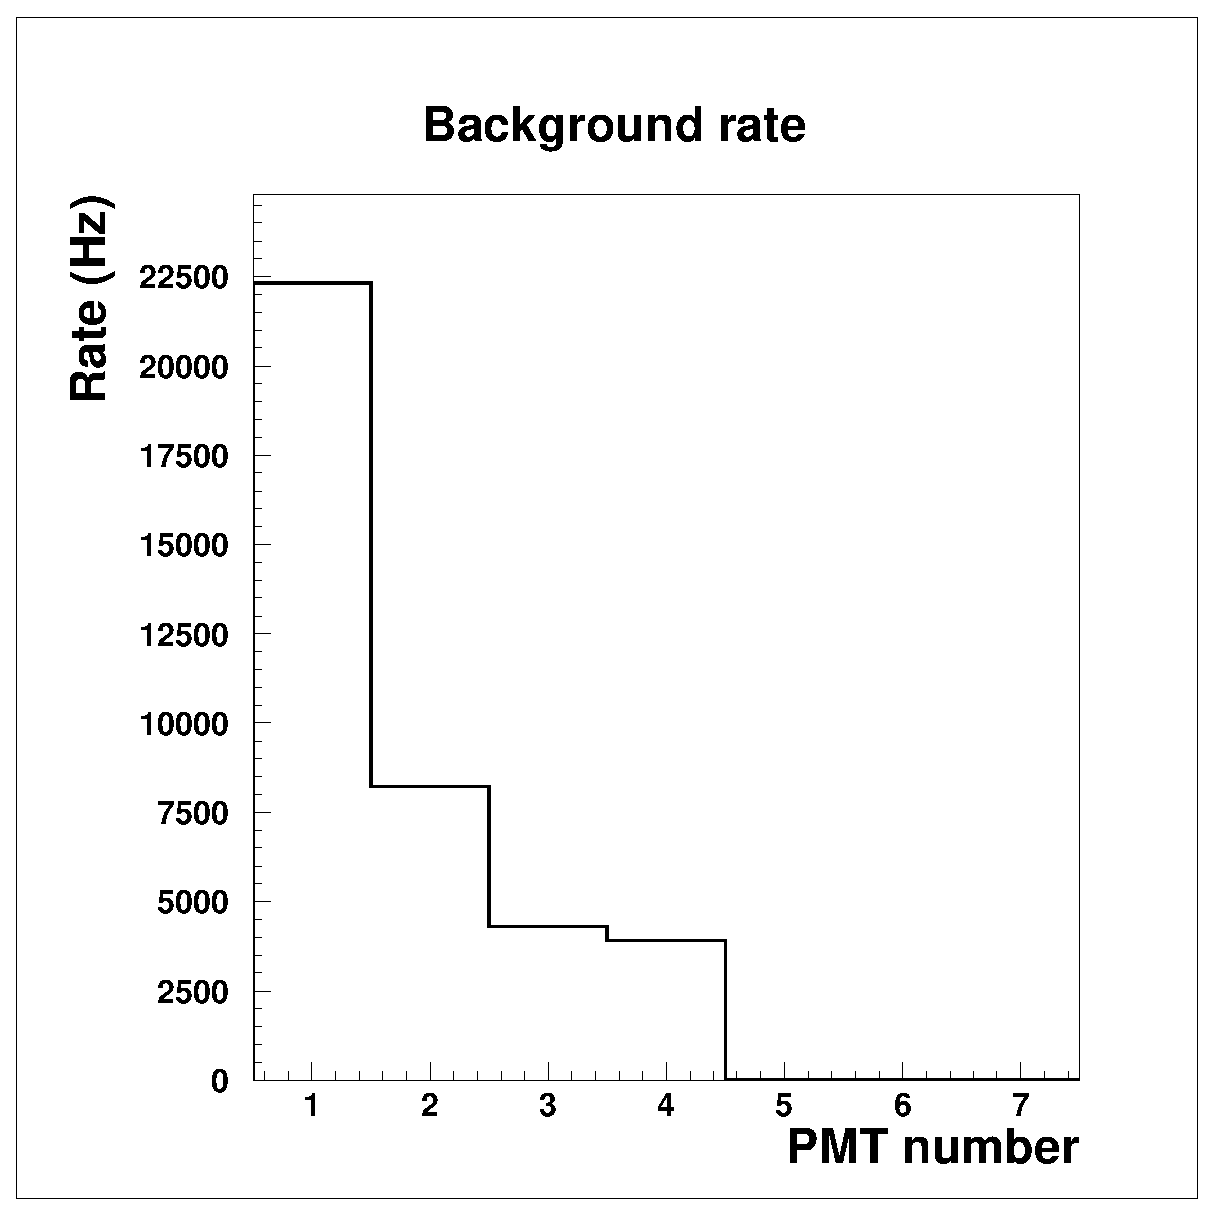
\includegraphics[height=6cm,angle=0]{MC-simulation/backgr2.eps}
\caption{\small{DVCS12 setup and background rates estimate.}}
\label{background2}
\end{figure}
%%%%%%%%%%%%%%%%%%%%%%%%%%%%%%%%%%%%%%%%%%%%%%%%%%%%%%%%%%%%%%%%%%%%%%

%%%%%%%%%%%%%%%%%%%%%%%%%%%%%%%%%%%%%%%%%%%%%%%%%%%%%%%%%%%%%%%%%%%%%%
%\begin{figure}[htbp]
%\centering
%\includegraphics[height=6cm,angle=0]{MC-simulation/dvcs12setup.eps}
%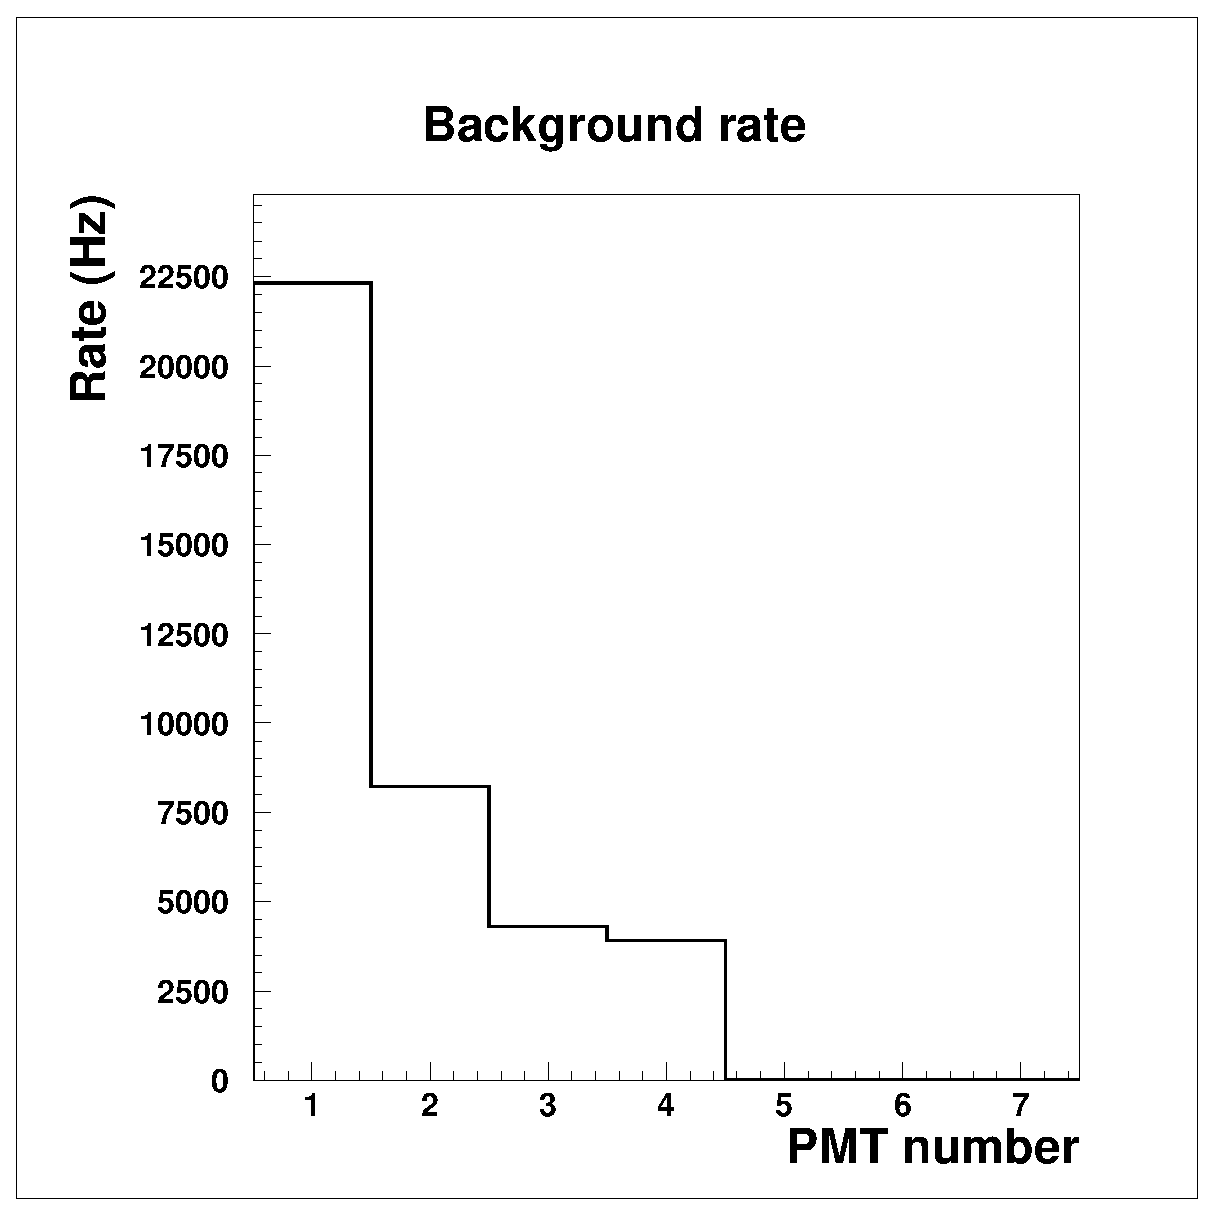
\includegraphics[height=6cm,angle=0]{MC-simulation/backgr2.eps}
%\caption{\small{The experimental setup and background rate estimate 
%(case 2).}}
%\label{background2}
%\end{figure}
%%%%%%%%%%%%%%%%%%%%%%%%%%%%%%%%%%%%%%%%%%%%%%%%%%%%%%%%%%%%%%%%%%%%%%

%%%%%%%%%%%%%%%%%%%%%%%%%%%%%%%%%%%%%%%%%%%%%%%%%%%%%%%%%%%%%%%%%%%%%%
\begin{figure}[htbp]
\centering
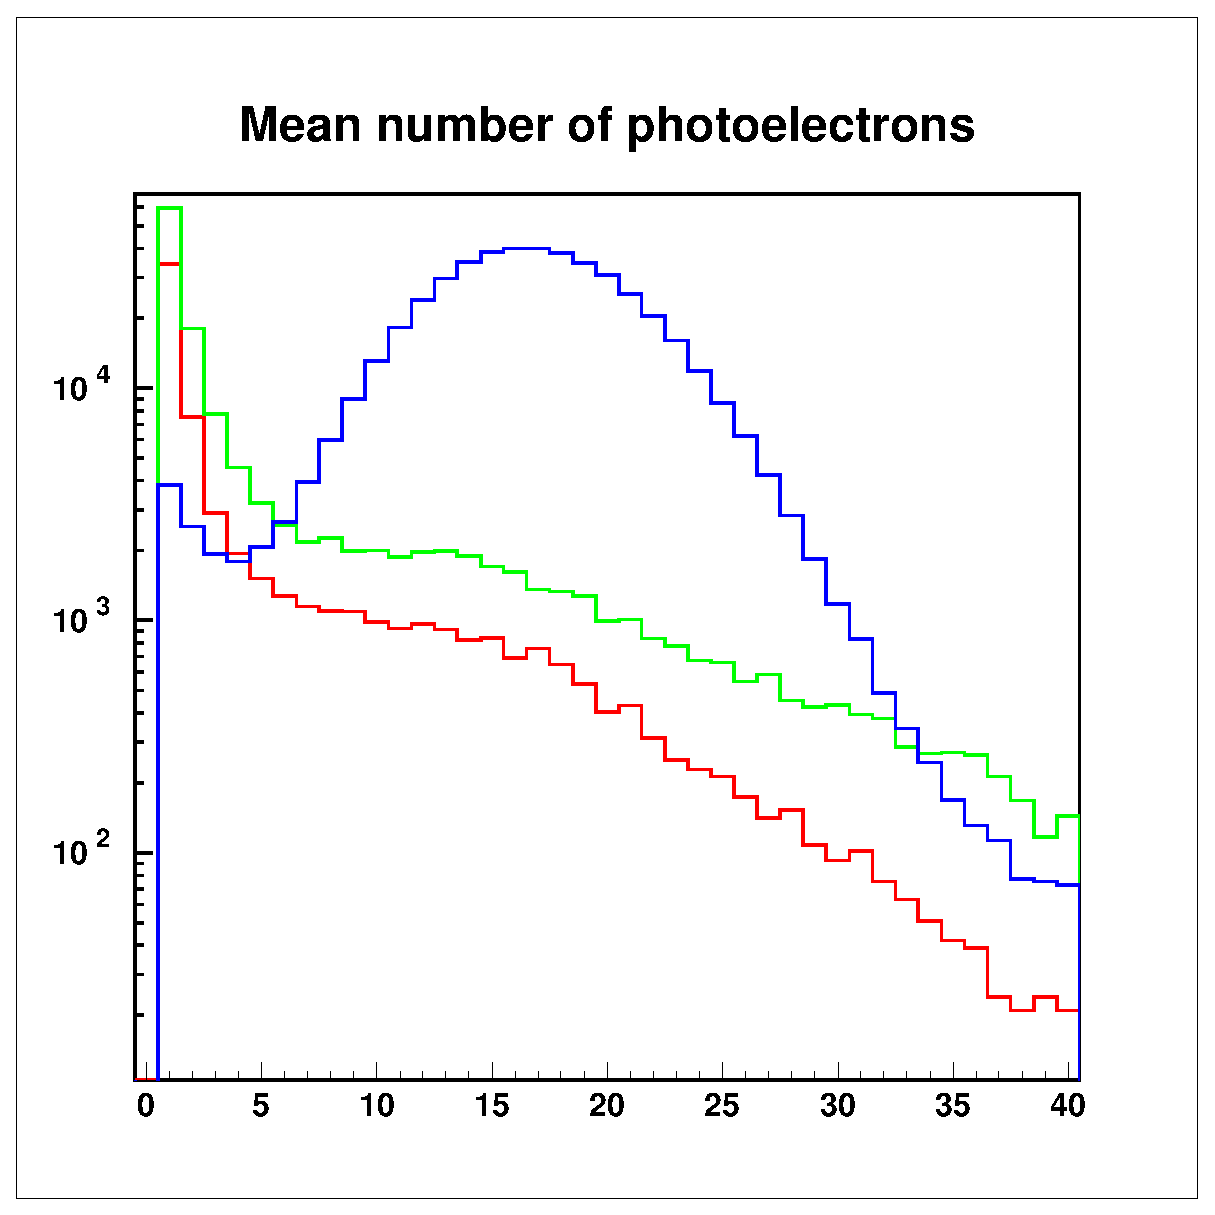
\includegraphics[height=8cm,angle=0]{MC-simulation/pions_nphe.eps}
\caption{\small{The amplitude distribution of detected pions (in 
photoelectrons) for 2~GeV (red curve) and 4~GeV pions (green curve).
The blue curve shows the amplitude distribution for the detected electrons.}}
\label{pions_nphe}
\end{figure}
%%%%%%%%%%%%%%%%%%%%%%%%%%%%%%%%%%%%%%%%%%%%%%%%%%%%%%%%%%%%%%%%%%%%%%

%%%%%%%%%%%%%%%%%%%%%%%%%%%%%%%%%%%%%%%%%%%%%%%%%%%%%%%%%%%%%%%%%%%%%%
\begin{figure}[htbp]
\centering
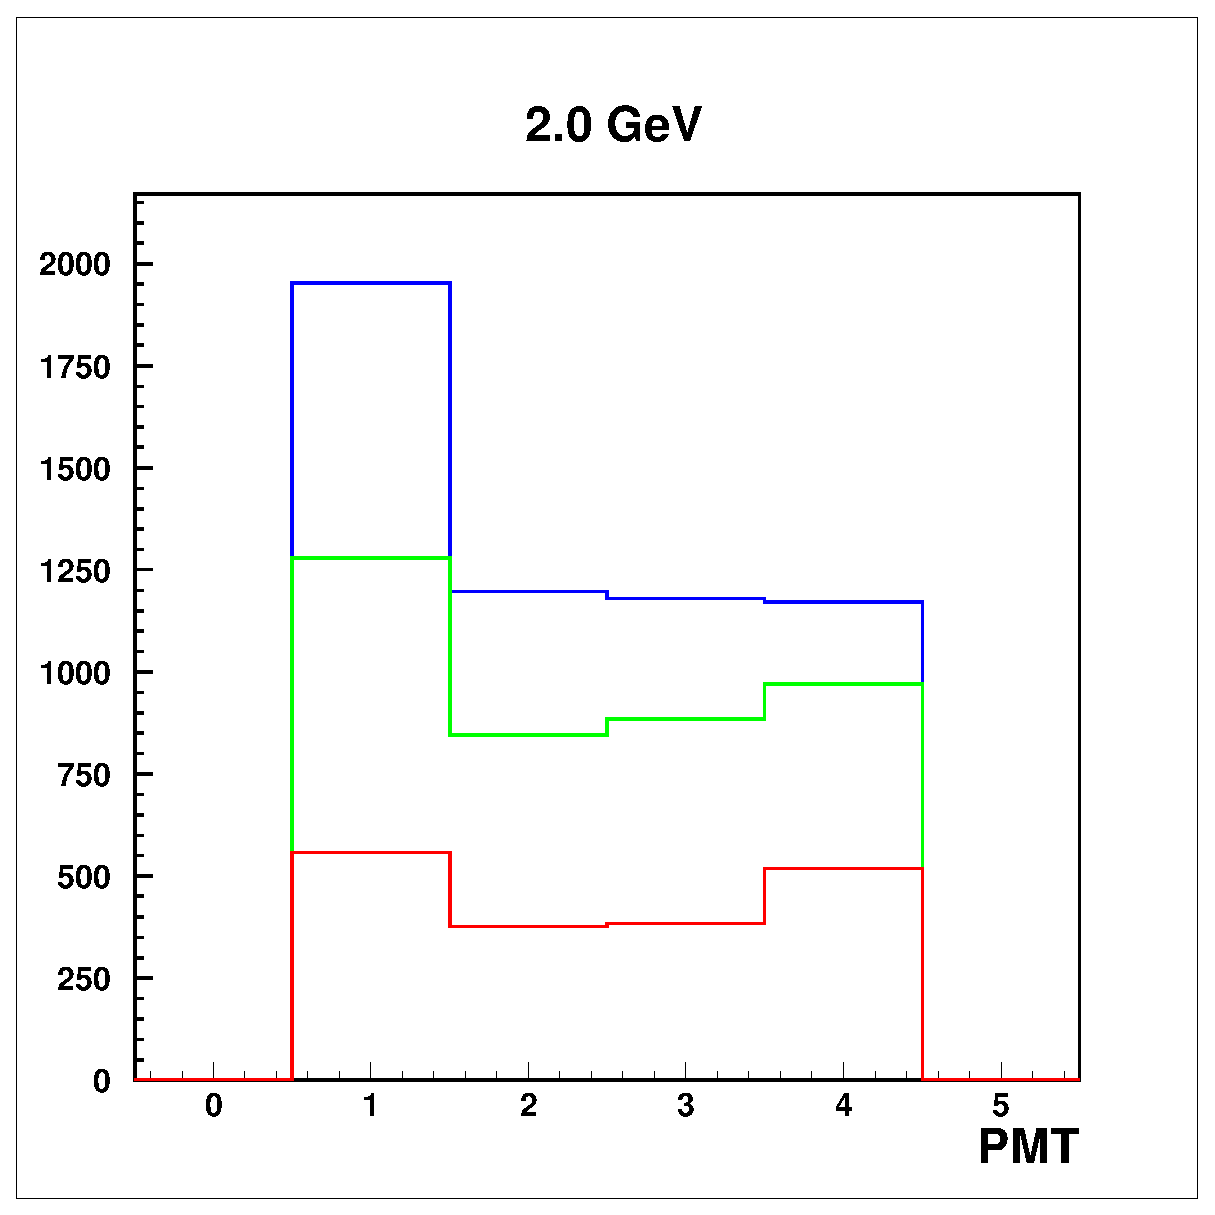
\includegraphics[height=8cm,angle=0]{MC-simulation/pions1a.eps}
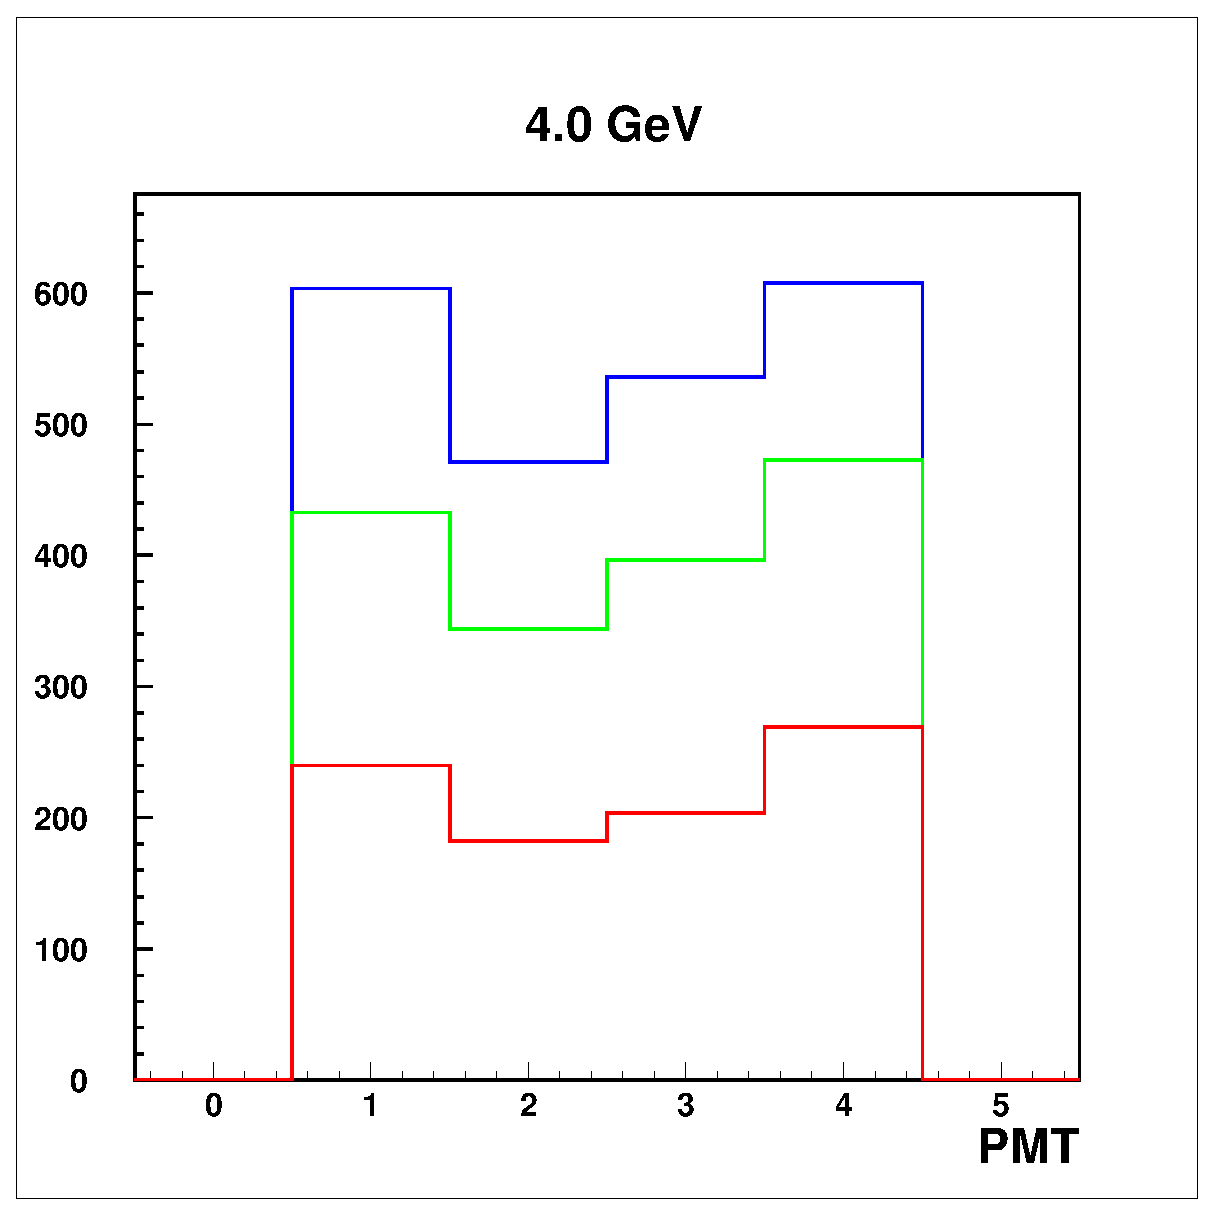
\includegraphics[height=8cm,angle=0]{MC-simulation/pions1b.eps}
\caption{\small{The simulated pion rejection factor of pions to electron 
identification for initial 2~GeV and 4~GeV pions.  The different curves 
represent different amplitude thresholds: red is for one photoelectron, 
green for two photoelectrons, and blue for three photoelectrons.}}
\label{pion-rejection}
\end{figure}
%%%%%%%%%%%%%%%%%%%%%%%%%%%%%%%%%%%%%%%%%%%%%%%%%%%%%%%%%%%%%%%%%%%%%%

The $\pi/e$ rejection factor is very important for the {\v C}erenkov 
detector.  Pions can produce $\delta$-electrons, which can be detected in 
the HTCC.  However, the amplitude distribution of such events is low. 
Fig.~\ref{pions_nphe} shows the amplitude distribution of detected pions 
(in photoelectrons) for 2~GeV (blue curve) and 4~GeV pions (red curve).

Fig.~\ref{pion-rejection} shows the $\pi/e$ rejection factor, calculated as 
the ratio of electron to pion detection efficiency, for 2~GeV and 4~GeV 
pions.  The red line shows the $\pi/e$ rejection factor with a threshold 
of one photoelectron, green - two photoelectrons, and blue - three 
photoelectrons.  The $\pi/e$ rejection factor can be as high as 500 even 
for high momentum pions.  It must be noted that the electron detection 
efficiency is still very high at thresholds up to three photoelectrons: 
99.99\% for two photoelectrons and 99.90\% for three photoelectrons.

\subsection{Timing Parameters}

GEANT can be used to estimate the trajectory length and the ray-tracing 
length difference for {\v C}erenkov photons for different PMTs.  The 
detection time difference is shown in Fig.~\ref{timing}.  It is evident 
that HTCC signals can be used for good time-of flight measurements, because 
even at larger $\theta$ angles, the timing is within $\pm$0.2~ns.

%%%%%%%%%%%%%%%%%%%%%%%%%%%%%%%%%%%%%%%%%%%%%%%%%%%%%%%%%%%%%%%%%%%%%%
\begin{figure}[htbp]
\centering
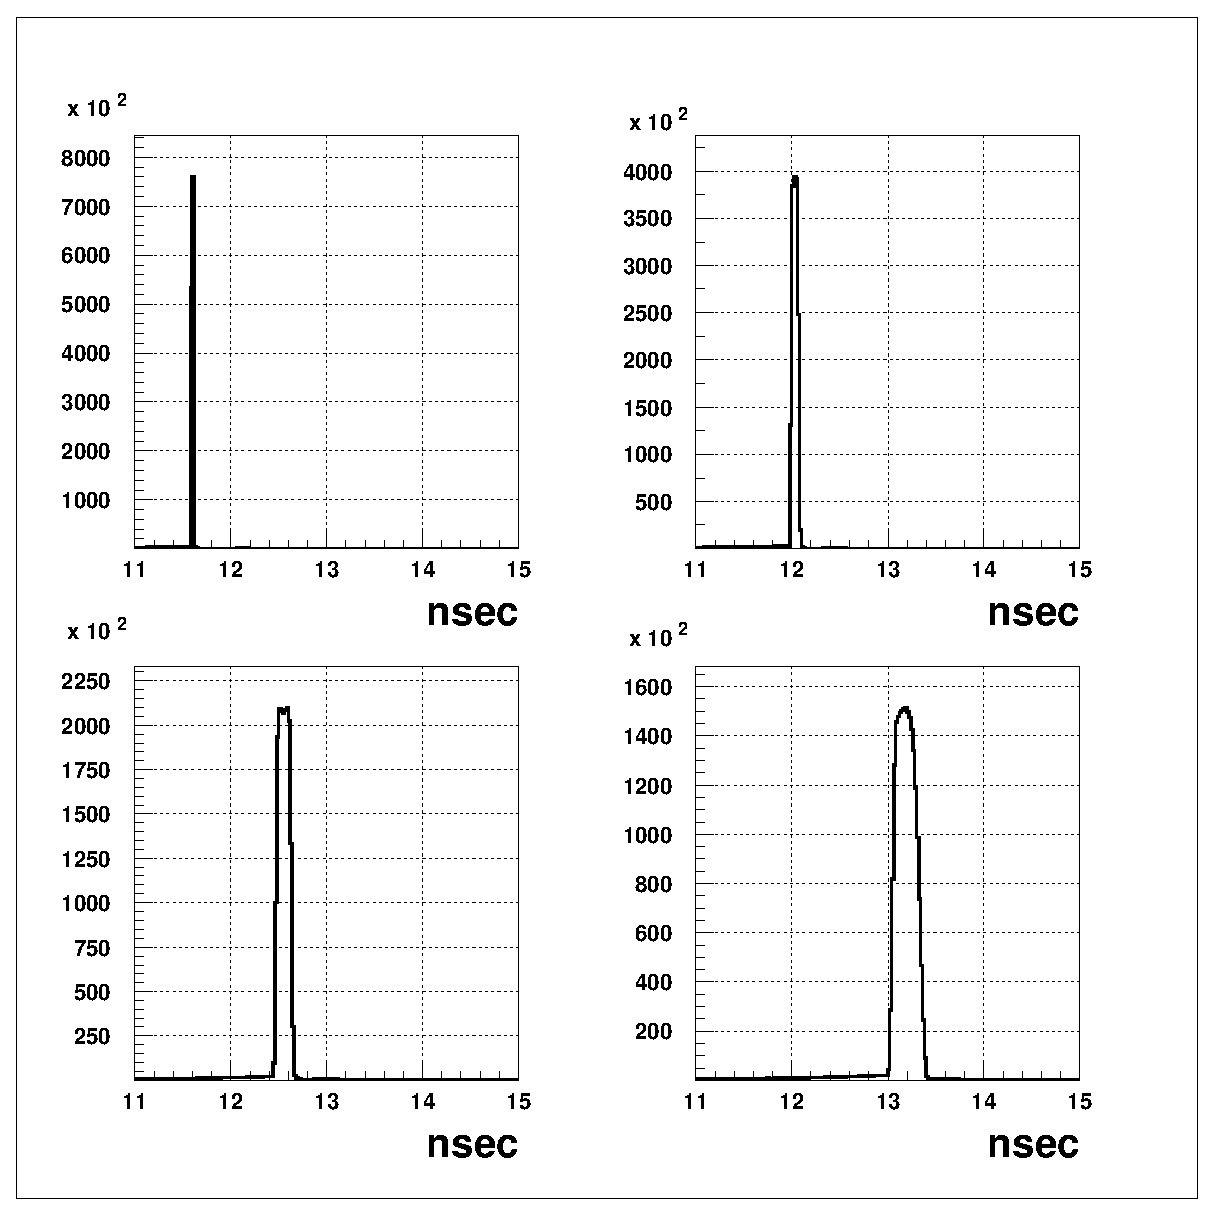
\includegraphics[height=10cm,angle=0]{MC-simulation/timing.eps}
\caption{\small{ The detection time difference for different HTCC PMTs.}}
\label{timing}
\end{figure}
%%%%%%%%%%%%%%%%%%%%%%%%%%%%%%%%%%%%%%%%%%%%%%%%%%%%%%%%%%%%%%%%%%%%%%
